\section{Software Implementation}

\subsection{Key Implementation Decisions}
\label{sec:kid}
In this section, the tools used for the implementation for this project have been detailed, and the reasons for their adoption have been justified.

\subsubsection{Implementation Platform - Responsive Web Application}
Responsive web applications have many advantages that make them perfect for this project. Firstly, they work both on desktop devices, and on mobile devices. This means that the application can be built one, and it will work (almost automatically) on both platforms, and therefore the user is not restricted to using only one. Further to this, a web application is ran through a web browser, and therefore there is no need to compensate for different operating systems or environments, as the application should theoretically work on them all. Another reason for picking this medium is that they are written in the default web languages, and the backend can be any language desired, meaning that external developers are much more likely to be able to pick it up and begin working on it (rather than them being required to have specific knowledge on how to create Android or iOS applications). The final major advantage is that they do not need to be downloaded, which means the user doesn't need to make a commitment to the application, and updates can be released instantaneously, and with ease. 

\subsubsection{Back End Tool - The Zend Framework (PHP)}
The back end tool of choice was the Zend Framework, which is written in PHP. This framework was picked because of its maturity, which includes its extensive documentation, online support, and well defined standards. This means an external developer can easily interpret the code produced, and can find help online if necessary. The Zend Framework also defines a very strict standard in how code should be organised and managed which is very intuitive to pick up, and helps split up large projects into small segments which are much more manageable. In addition to this, the development of a Zend application can be heavily sped up with the use of its many convenience classes and extra features, such as form generation and validation, and authentication. This also has the advantage that it is well documented by Zend themselves, and help is easily accessible, which will help future developers to understand and debug the code.

\subsubsection{Front End Tool - Twitter's Bootstrap}
Twitter's Bootstrap is extremely well known and extremely well documented. This makes it very simple for new users to understand how it works, and how to start using it themselves. It effortlessly creates aesthetically pleasing websites, with little work required on the part of the developer, which makes it perfect for a project like this. In addition to this, it automatically resizes to different screen sizes and display resolutions, which is a necessity for a responsive web application.\ \\
\ \\
One important factor that was taken into consideration when designing the site was how to make it stand out from other websites developed with Bootstrap. The main step was to use a flat design with special orange highlights to give the site a unique defining feature and colour scheme, which helps to make it distinguishable from other Bootstrap websites. In addition to this, other libraries were also used, like the jquery-confirm\footnote{\url{http://craftpip.github.io/jquery-confirm/}} plugin, instead of some of Bootstrap's default features (like modals), to further help it stand out.

\newpage 
\subsection{Implementation Methodology}
For a project of this size, it was a necessity to define some standards for how work would be completed. I decided to use an agile approach, utilising a Kanban board, and to work with the tips laid out by Henrik Kniberg\cite{kniberg2007scrum}. The main reason for this is that it allowed for quick pivoting of focus (when bugs arose), I had a lot of experience with it already (having used it for my last large project) and found I worked well under its regime. At the beginning of the project, the list of requirements was generated from the specification sent by the client. This list was then broken down into different core components of the site (route creation, route discovery, etc), and then each individual task broken down into subtasks. Each of these subtasks was then put on a digital Kanban board, using a service called Trello\footnote{\url{http://www.trello.com}} (combined with the extension Scrum for Trello\footnote{\url{https://q42.com/projects}} to add extra scrum functionality, like time estimations), to keep track of their progress, and for scheduling. The main advantage of splitting each task into many smaller subtasks, is that it meant it was easy to make progress on the project every day, as these tasks did not (individually) take a long time to complete. It also meant that no tasks were ever forgotten about, and bugs could easily be recorded and resolved. It has been shown that it is easier to reach goals if they have been explicitly written and expressed\cite{wilson2008goal}, which is why this Kanban method was so successful, especially as this could be shared with my project supervisor.

\begin{figure}[!ht]
	\vspace{2mm}
	\begin{center}
		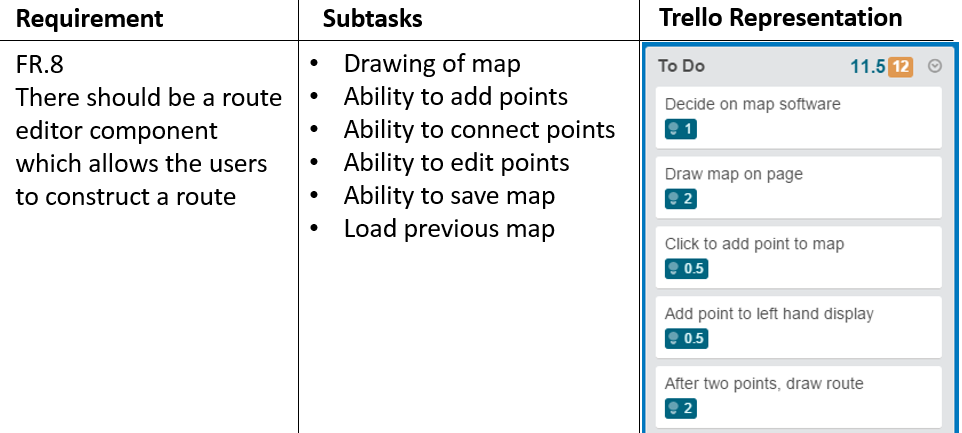
\includegraphics[width=0.8\textwidth]{images/implementation/task_breakdown.png}
	\end{center}
	\vspace{-6mm}
	\caption{Process for breaking down tasks, adding extra granularity with each step}
	\vspace{-10mm}	
\end{figure}
\ \\
\ \\
At the beginning of each week (where a week started on the day of project supervision meetings) the total list of tasks to be completed was evaluated. Based on priorities, prerequisites, and the Gantt chart produced for the project proposal (displayed in appendix \ref{sec:gantt}), a group of tasks would be selected for completion that week. Each task was given an estimated time of completion which would be used in conjunction with the number of work hours completed in the previous week to decide how many tasks should be picked. This meant that a constant stream of work was completed every week, and that the project did not fall behind. Having weekly meetings was extremely useful, as they were a chance to course-correct if things weren't going to plan, to receive feedback on the progress of the project, and to get an outside perspective on how new features looked and behaved.

\newpage 
\subsection{Problems Encountered}
\label{sec:problems}
Assuming that a large project could be completed without any problems or issues along the way would be foolish, and this project was certainly no different. It is, therefore, extremely important to identify what these problems are, what the causes were, and how these can be prevented in the future. The biggest problem faced during the implementation of Niceway.to, was the lack of a proper testing framework. As new features were added, they were individually tested, and some minor integration testing was carried out with other parts of the system they may have had an impact on. After this was done, the feature was assumed to be bug free, and progress on the project continued. However, on several occasions, a new feature would be added, tested briefly, and marked as complete, only to have it be the root cause of some problem further down the line, due to some unforeseen interaction with another component. This meant that a lot of time was dedicated to going back to previous features and fixing them, instead of pushing the project forward. The solution to this would be to implement unit testing on every aspect of the system. This would mean, after the addition of any features, a set of tests could be run to ensure that all components of the system are still functioning as expected. Considering how well integrated unit tests are with the Zend framework, their lack of inclusion is this project is even more worrying. The main reason for this is how some work on the project was prototyped before its official commencement. This prototyped code did not implement testing, and was later directly included in the project. This meant that the speed of the initial stages of the project were accelerated, but meant that unit tests were left out, and with such a large code base now, it would troublesome to implement them at this point.\ \\
\ \\
The next major problem encountered was the lack of proper research into an adequate routing service. When implementing the functionality to draw a route between two points, not much research was conducted into which routing service would be the best, and instead the easiest to implement was selected. This initial routing service was the MapBox default routing service, which was extremely easy to implement, because MapBox was being used to provide the map. After implementing the functionality to draw these routes, it became apparent that the service had a limit to the number of points it could route at any one time (a maximum of twelve), and that the service was unreliable (at times it would be unable to provide any route at all). This meant that a new service needed to be selected (the Leaflet Routing Machine), and that a lot of the functionality for routing needed to be rewritten with this new library. This wasted a lot of time, as work that was previous deemed complete needed to be completed a second time. This could have been resolved by expanding the research conducted at the beginning of the project, and being more thorough in which software was investigated (instead of just back end and front end tools, it would have been beneficial to look at libraries that were required as well). \ \\
\ \\
The third major problem was lack of attention to detail in the creation of the requirements. At the beginning of the project, the client provided a specification for the project, which included all features he required. This was then converted into a requirements specification, with functional and non-functional requirements. However, during this conversion, some of the intricate details of the initial specification were lost. This meant that, half way through the project, it was discovered that there was a large amount of functionality missing. Not only did this add extra pressure to the project, but also meant that many previous features had to be revisited and revised, which meant a lot of time had been wasted in the implementation procedure. In future, this can be avoided by paying much closer attention to the initial specification, and ensuring that all details are extracted as necessary, and getting the client to sign off on these extracted requirements.



